\Chapter{Wires and wireless}
\label{chap:wires-wireless}

\Section{Wires}
\label{sec:wires}

\Paragraph{twisted pair}
\mode<article>{
Twisted pair cabling is a type of wiring in which two conductors of a single circuit are twisted together for the purposes of improving electromagnetic compatibility.
Compared to a single conductor or an untwisted balanced pair, a twisted pair reduces electromagnetic radiation from the pair and crosstalk between neighbouring pairs and improves rejection of external \ac{EMI}.
It was invented by Alexander Graham Bell.
}

\Paragraph{shielded vs unshielded}
\mode<article>{
For additional noise immunity, twisted-pair cabling may be shielded.
Cable with shielding is known as \ac{ShTP} and without as \ac{UTP}.

Common shield construction types include \emph{individual} shielding (\abbr{U/\-FTP}) with aluminium foil for each twisted pair or quad.
This type of shielding helps prevent \ac{EMI} from entering or exiting individual pairs and also protects neighbouring pairs from crosstalk.
\emph{Overall} shielding with overall foil (\abbr{F/UTP}), braided shield (\abbr{S/UTP}), or braiding with foil across all of the pairs (\abbr{SF/UTP}).
This type of shielding helps prevent \ac{EMI} from entering or exiting the cable.

Finally, there is \emph{individual and overall} shielding which uses individual shielding using foil between the twisted pair sets, and also an outer foil or braided shielding (\abbr{F/FTP}, \abbr{S/FTP}, and \abbr{SF/FTP}).
This type of shielding helps prevent \ac{EMI} from entering or exiting the cable and also protects neighbouring pairs from crosstalk.
}

\Paragraph{categories}
\mode<article>{
There are different categories of twisted pair cabling.
Each category must adhere to a different standard and stringent specifications for crosstalk and system noise.
These standard specify the maximum distance a cable must be able to cover, the bandwidth, and the required shielding.

See \vref{tab:tp-categories} for an overview of the different categories.


\begin{table}
   \caption{Twisted pair categories}
   \label{tab:tp-categories}
   \centering
   \sffamily
   \begin{tabular}{lrrl}
   \textbf{cat.} & \textbf{dist. (m)} & \textbf{\textsc{BW} (MHz)} & \textbf{application} \\[1ex]
   3 & 100 & 16 & \abbr{10BASE-T} \\
   4 &     & 20 & Token Ring \\
   5 & 100 & 100 & \abbr{1000BASE-T} \\
   5e & 100 & 100 & \abbr{1000BASE-T}, \abbr{2.5GBASE-T} \\
   6  & 55  & 250 & \abbr{10GBASE-T} \\
   $6_\mathrm{A}$ & 100 & 500 & \abbr{10GBASE-T} \\
   7 & 100 & 600 & \abbr{10GBASE-T} \\
   $7_\mathrm{A}$ & & 1000 & \\
   8.1 & 36 & 2000 & \abbr{40GBASE-T} \\
   8.2 & 36 & 2000 & \abbr{40GBASE-T} \\
   \end{tabular}
\end{table}
}

\Paragraph{\acs{RJ45}}
\mode<article>{
The connector used for network cables is actually called an \acs{8P8C} connector but everyone knows it as a \acs{RJ45} connector.
A completely plastic connector is used for unshielded cabling while a metalic version exists for shield cabling.

\begin{figure}
   \centering
   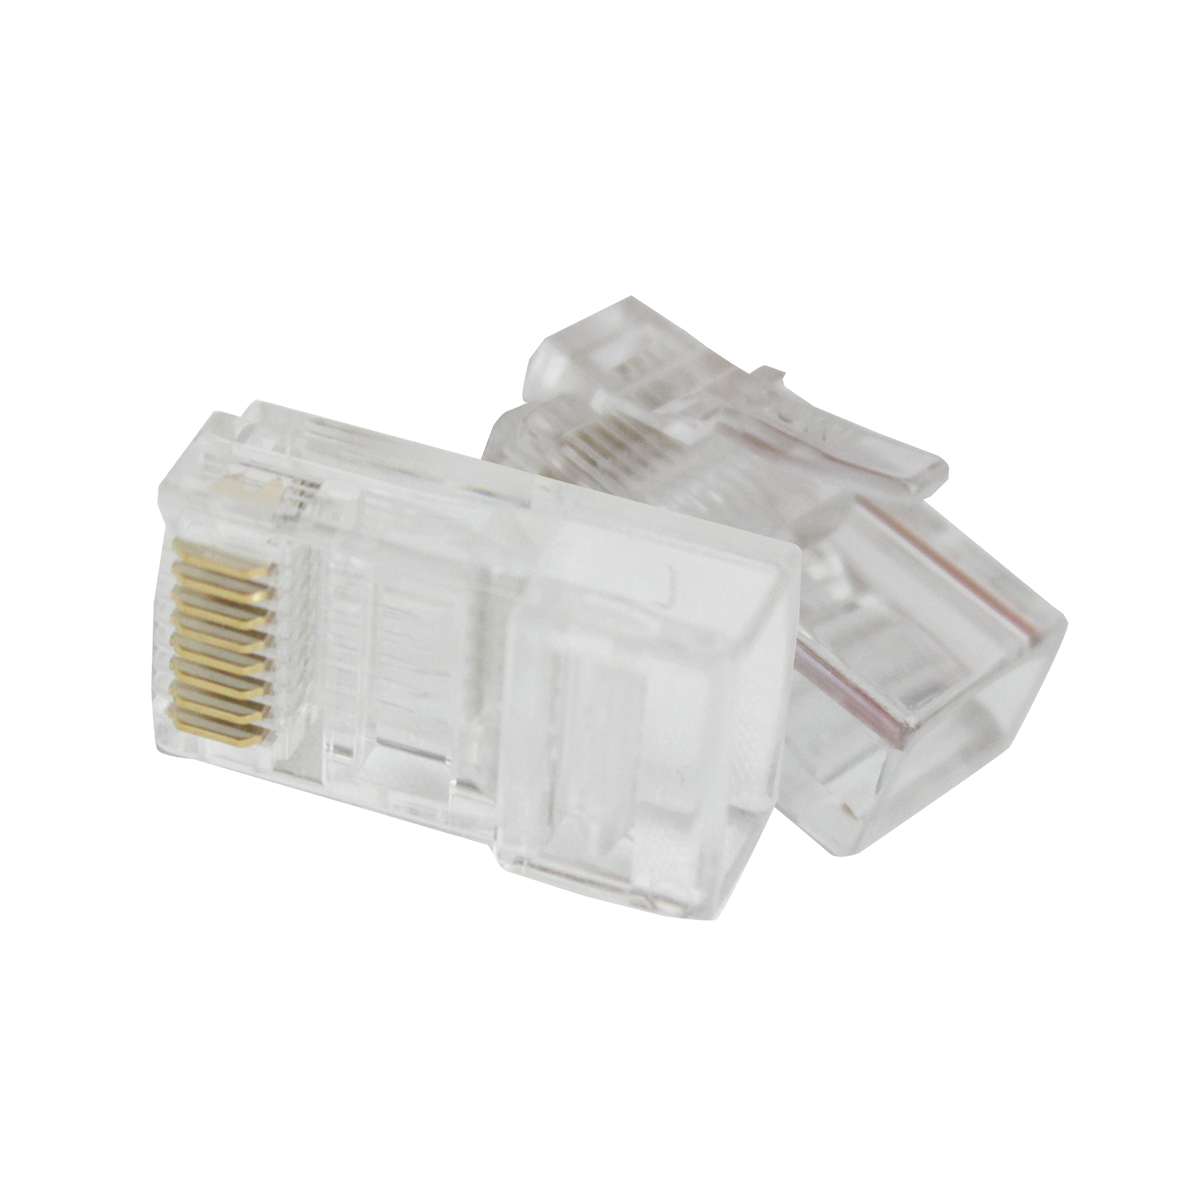
\includegraphics[width=.5\textwidth]{images/8p8c.png}
   \caption{Two plastic \acs{RJ45} connectors used with unshielded cabling}
   \label{fig:rj45}
\end{figure}
}
\slide{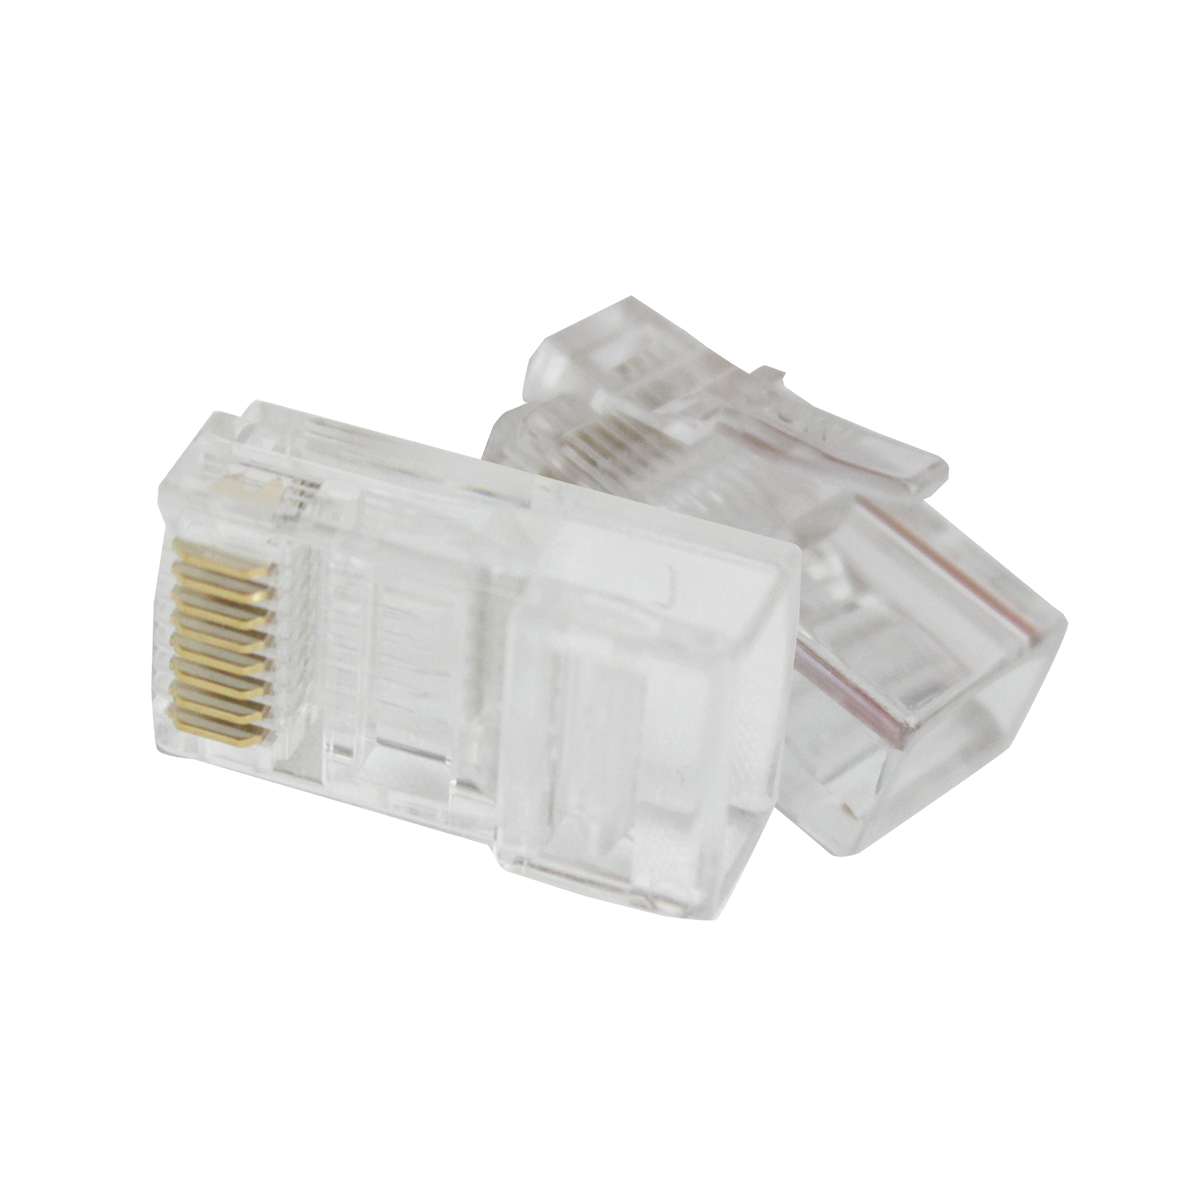
\includegraphics[width=.7\textwidth]{images/8p8c.png}}

\Paragraph{Fast Ethernet}
\mode<article>{
\abbr{100BASE-TX} is the predominant form of Fast Ethernet, and runs over two wire-pairs inside a category~5 or above cable.
Each network segment can have a maximum cabling distance of \SI{100}{\metre}.
One pair is used for each direction, providing full-duplex operation with \SI{100}{\mega\bit\per\second} of throughput in each direction.
Like \abbr{10BASE-T}, the active pairs in a standard connection are terminated on pins 1,~2,~3 and~6.
Since a typical category~5 cable contains 4~pairs, it can support two \abbr{100BASE-TX} links with a wiring adaptor.
}

\Paragraph{crossover cable}
\mode<article>{
An Ethernet crossover cable is a crossover cable for Ethernet used to connect computing devices together directly.
It is most often used to connect two devices of the same type, e.g. two computers (via their network interface controllers) or two switches to each other.
By contrast, \emph{straight-through} patch cables are used to connect devices of different types, such as a computer to a network switch.
Intentionally crossed wiring in the crossover cable connects the transmit signals at one end to the receive signals at the other end.
Many network devices today support auto-\acs{MDI-X} (aka auto-crossover) capability, wherein a patch cable can be used in place of a crossover cable, or vice versa, and the receive and transmit signals are reconfigured automatically within the device to yield a working connection.

To make a straight-through patch cable, either use the order defined by \abbr{T568A} on both ends of the cable, or the order defined by \abbr{T568B}.
To create a crossover patch cable, use \abbr{T568A} on one side and \abbr{T568B} on the other.

\begin{figure}
\centering
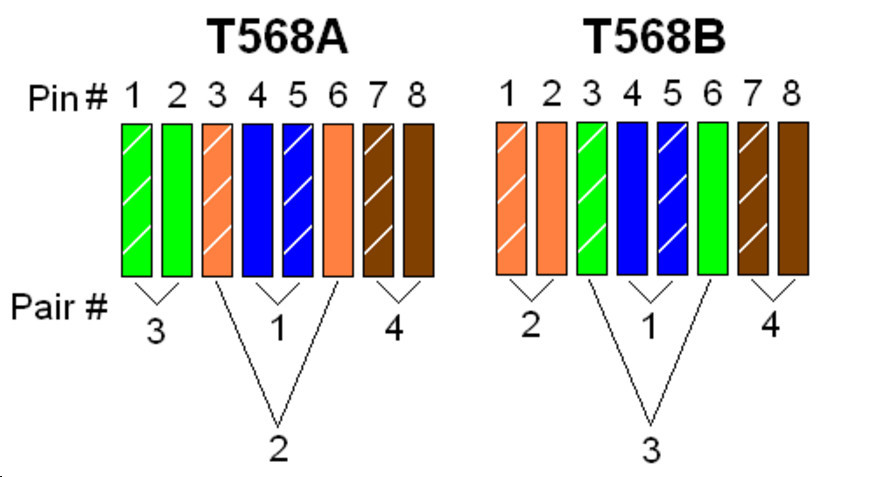
\includegraphics[width=.7\textwidth]{images/t568.jpeg}
\caption{The \abbr{T568} standard for twisted-pair cabling}
\label{fig:t568}
\end{figure}

% TODO: explain (with a drawing?) that pair 1/3 is used for sending and the other for receiving data.
}

\Paragraph{Gigabit Ethernet}
\mode<article>{
In computer networking, Gigabit Ethernet (GbE or 1~GigE) is the term applied to transmitting Ethernet frames at a rate of a gigabit per second.
The most popular variant \abbr{1000BASE-T} is defined by the \acs{IEEE} 802.3ab standard.
It came into use in 1999, and has replaced Fast Ethernet in wired local networks due to its considerable speed improvement over Fast Ethernet, as well as its use of cables and equipment that are widely available, economical, and similar to previous standards.

Each \abbr{1000BASE-T} network segment is recommended to be a maximum length of 100~metres, and must use Category~5 cable or better (including Cat~5e and Cat~6).
In a departure from both \abbr{10BASE-T} and \abbr{100BASE-TX}, \abbr{1000BASE-T} uses four lanes over all four cable pairs for simultaneous transmission in both directions.
}

\Paragraph{auto \acs{MDI-X}}
\mode<article>{
Auto \acs{MDI-X} (aka `auto crossover') automatically detects the required cable connection type and configures the connection appropriately, removing the need for crossover cables to interconnect switches or connecting \acsp{PC} peer-to-peer.
As long as it is enabled on either end of a link, either type of cable can be used.
For auto \acs{MDI-X} to operate correctly, the data rate on the interface and duplex setting must be set to `auto.'

Gigabit and faster Ethernet links over twisted pair cable use all four cable pairs for simultaneous transmission in both directions.
For this reason, there are no dedicated transmit and receive pairs, and consequently, crossover cables are never required for \abbr{1000BASE-T} communication.
}

\Paragraph{100\,Gbit Ethernet}
\mode<article>{
Using Cat.~8 twisted pair cabling it is possible to go up to \SI{40}{\giga\bit\per\second} using cables up to \SI{30}{\metre}.
Higher speeds or longer lengths require fibre optic cables to be used.
}

\Paragraph{\acl{DAC}}
\mode<article>{
A \acf{DAC} cable is a copper 10~Gigabit Ethernet cable which comes in either an active or passive twinax (twinaxial) cable assembly and connects directly into an \acs{SFP+} housing (\vref{fig:dac}).
\abbr{40GBASE-CR4} and \abbr{100GBASE-CR10} physical layers using \SI{7}{\metre} twin-axial cable are being developed as part of the 100~Gbit Ethernet specifications by the \acs{IEEE}.

\begin{figure}
\centering
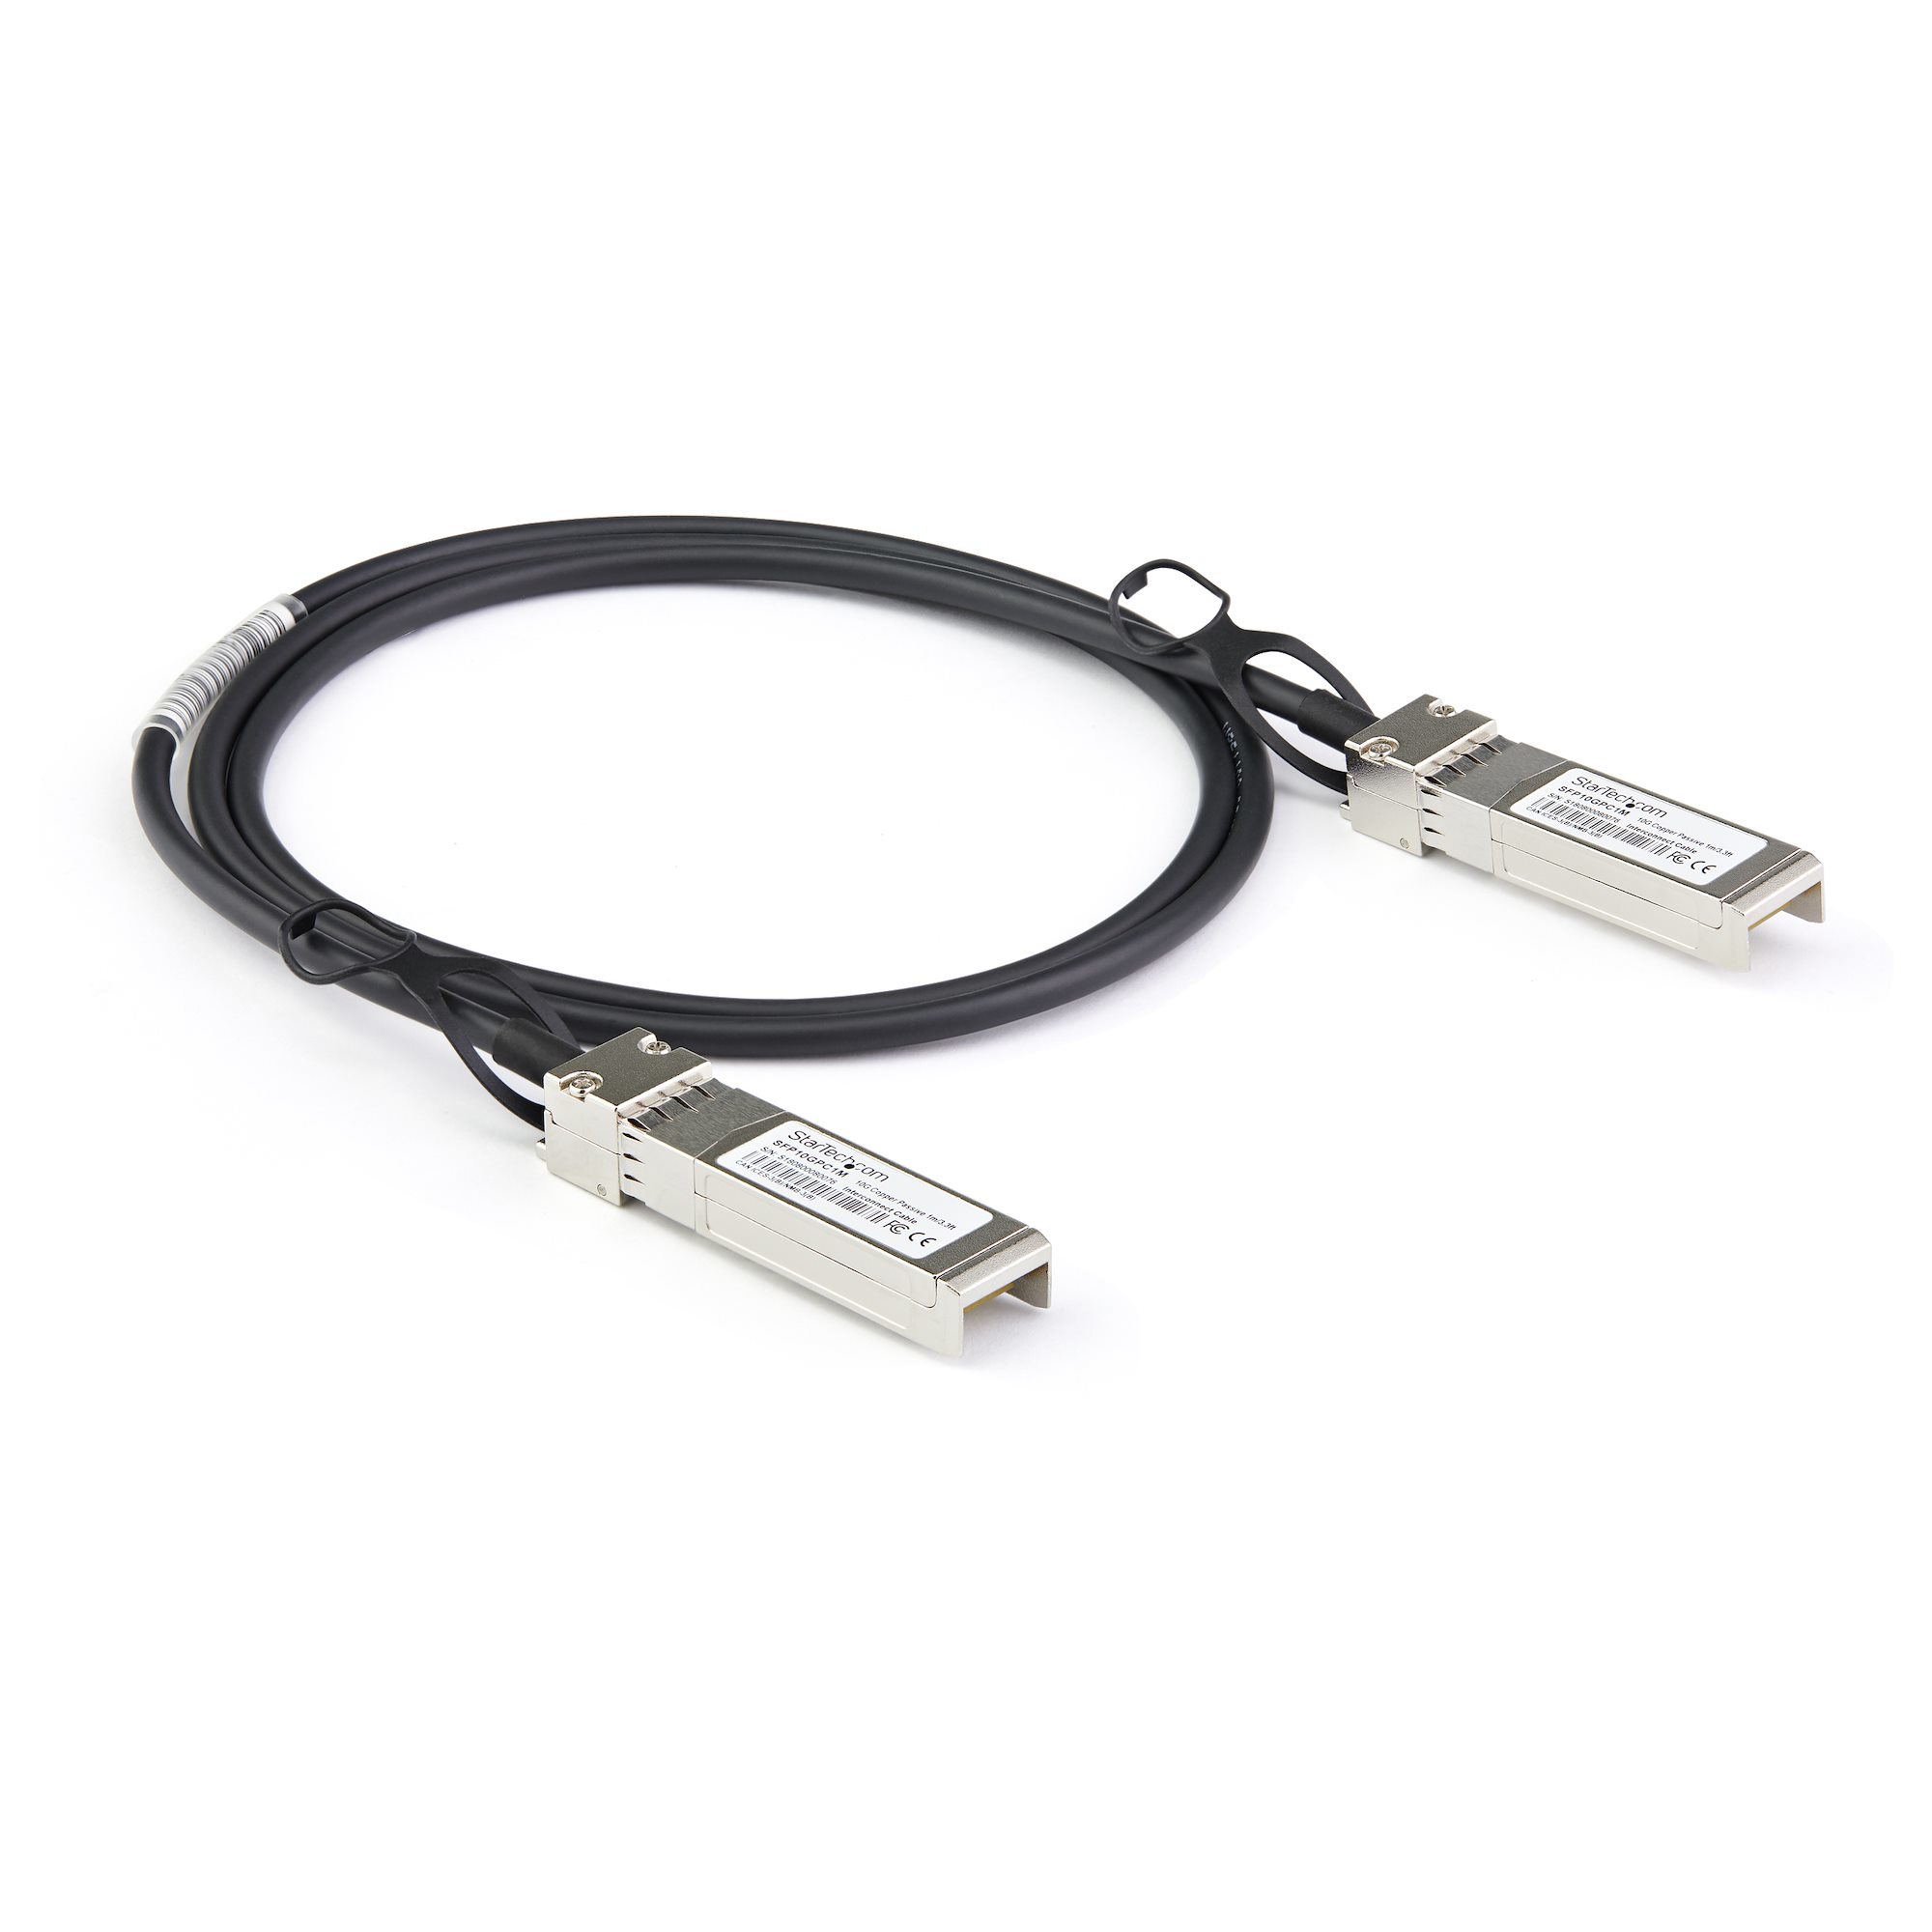
\includegraphics[width=.7\textwidth]{images/dac-cable.jpeg}
\caption{A direct-attach copper cable}
\label{fig:dac}
\end{figure}
}

\Paragraph{optical fibre}
\mode<article>{
An optical fibre is a flexible, transparent fibre made by drawing glass (silica) or plastic to a diameter slightly thicker than that of a human hair.
Fibres are used instead of metal wires because signals travel along them with less loss; in addition, fibres are immune to electromagnetic interference, a problem from which metal wires suffer.
The concept of a direct-attech copper cable also exist with optical cables.
These are then called \acf{AOC}.

\begin{table}
   \caption{Fibre optic categories}
   \label{tab:fo-categories}
   \centering
   \sffamily
   \begin{tabular}{lrrll}
   \textbf{cat.} & \textbf{core ($\bm{\mathrm{\upmu{}m}}$)} & {\small\textbf{\abbr{BW} (MHz)}} & \textbf{color} & \textbf{Ethernet standard} \\[1ex]
   \abbr{OM1} & 62.5    &  200 & orange & {\small \abbr{10GBASE-SR} (\SI{33}{\metre})} \\
   \abbr{OM2} & 50      &  500 & orange & {\small \abbr{10GBASE-SR} (\SI{82}{\metre})} \\
   \abbr{OM3} & 50      & 2000 & aqua   & {\small \abbr{100GBASE-SR4} (\SI{100}{\metre})} \\
   \abbr{OM4} & 50      & 4700 & aqua   & {\small \abbr{100GBASE-SR4} (\SI{150}{\metre})}\\
   \abbr{OS1} & 8--10.5 &      & yellow & {\small \abbr{100GBASE-ER4} (\SI{40}{\kilo\metre})} \\
   \abbr{OS2} & 8--10.5 &      & yellow & {\small \abbr{100GBASE-ER4} (\SI{40}{\kilo\metre})} \\
   \end{tabular}
\end{table}
}

\Paragraph{single-mode}
\mode<article>{
In fibre-optic communication, a \ac{SMF}, also known as fundamental- or mono-mode, is an optical fibre designed to carry only a single mode of light -- the transverse mode.
Waves can have the same mode but have different frequencies. This is the case in single-mode fibres, where we can have waves with different frequencies, but of the same mode, which means that they are distributed in space in the same way, and that gives us a single ray of light.
}

\Paragraph{multi-mode}
\mode<article>{
Multi-mode optical fibre is a type of optical fibre mostly used for communication over short distances, such as within a building or on a campus.
Multi-mode links can be used for data rates up to \SI{100}{\giga\bit\per\second}.
Multi-mode fibre has a fairly large core diameter that enables multiple light modes to be propagated and limits the maximum length of a transmission link because of modal dispersion.
}

\Paragraph{transceivers}
\mode<article>{
As there are so many different options regarding transceivers depending on bandwidth, distance and the use of lasers or \acsp{LED}, network equipment does not have built-in transceivers.
It is more convenient to have a modular system where you can plug in the transceiver you need.
There are different form factors available, including \acs{SFP}, \acs{SFP+} and \acs{QSFP}.

\begin{figure}
   \begin{subfigure}[b]{0.45\textwidth}
   \centering
   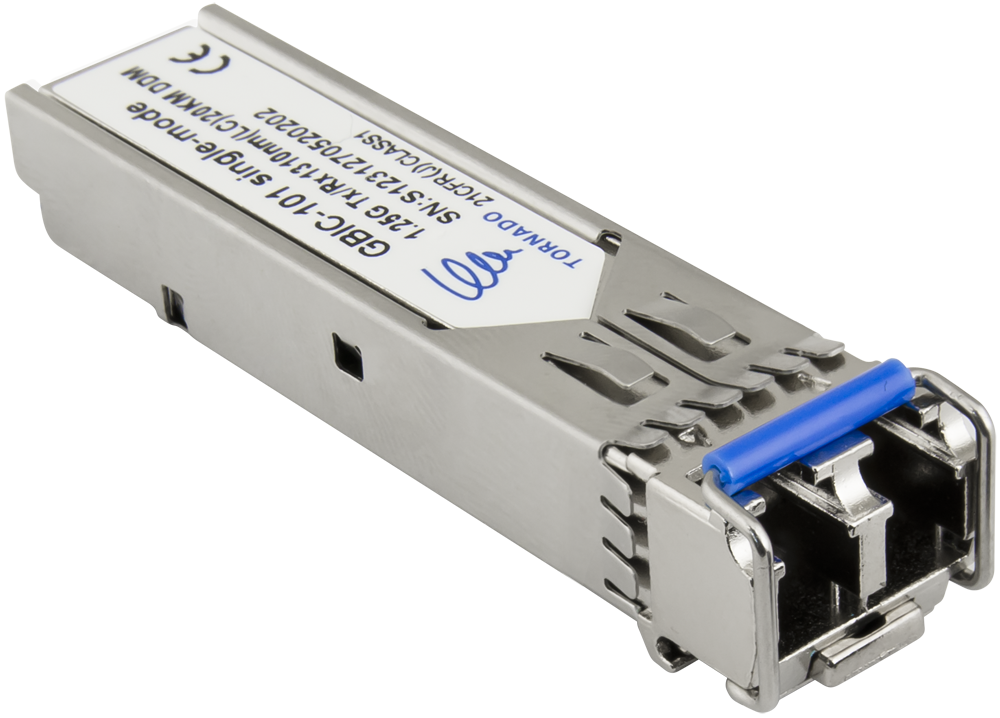
\includegraphics[width=\textwidth]{images/sfp.png}
   \caption{An \acs{SFP} with an \acs{LC} connector}
   \label{fig:sfp-lc}
   \end{subfigure}
   \hfill
   \begin{subfigure}[b]{0.45\textwidth}
   \centering
   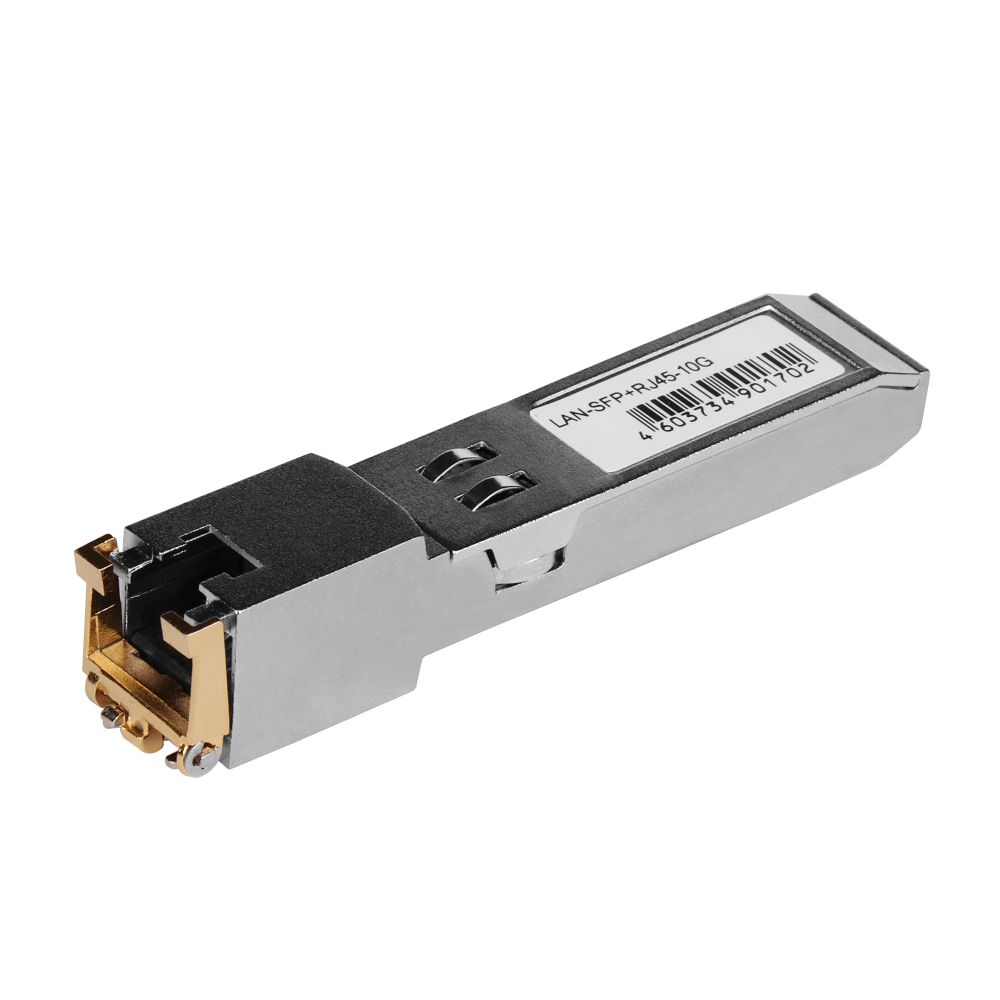
\includegraphics[width=\textwidth]{images/sfp-rj45.png}
   \caption{An \acs{SFP} with a \acs{RJ45} connector}
   \label{fig:sfp-rj45}
   \end{subfigure}
   \caption{Two small \acf{SFP} transceivers}
   \label{fig:sfp}
\end{figure}

Nowadays most connectors are \acs{LC} (as in \vref{fig:sfp}) but in data centres \acs{MPO} cables (\vref{fig:mpo}) are also used for high-speed connections and for interconnecting patch panels.
An \acs{MPO} cable can have up to 72 fibre strands in a cable.
See also \href{https://www.qsfptek.com/article/fiber-connector-types-lc-sc-fc-st-mtp-mpo}{qsfptek.com} for more information on different fibre optic connectors.

\begin{figure}
   \centering
   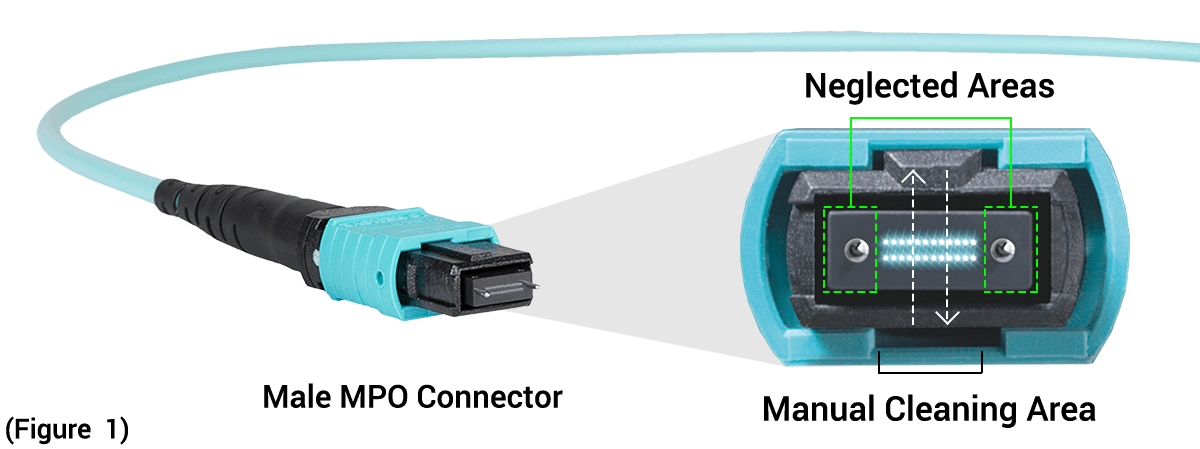
\includegraphics[width=\textwidth]{images/mpo.png}
   \caption{\acs{MPO} connnector}
   \label{fig:mpo}
\end{figure}

\begin{figure}
   \centering
   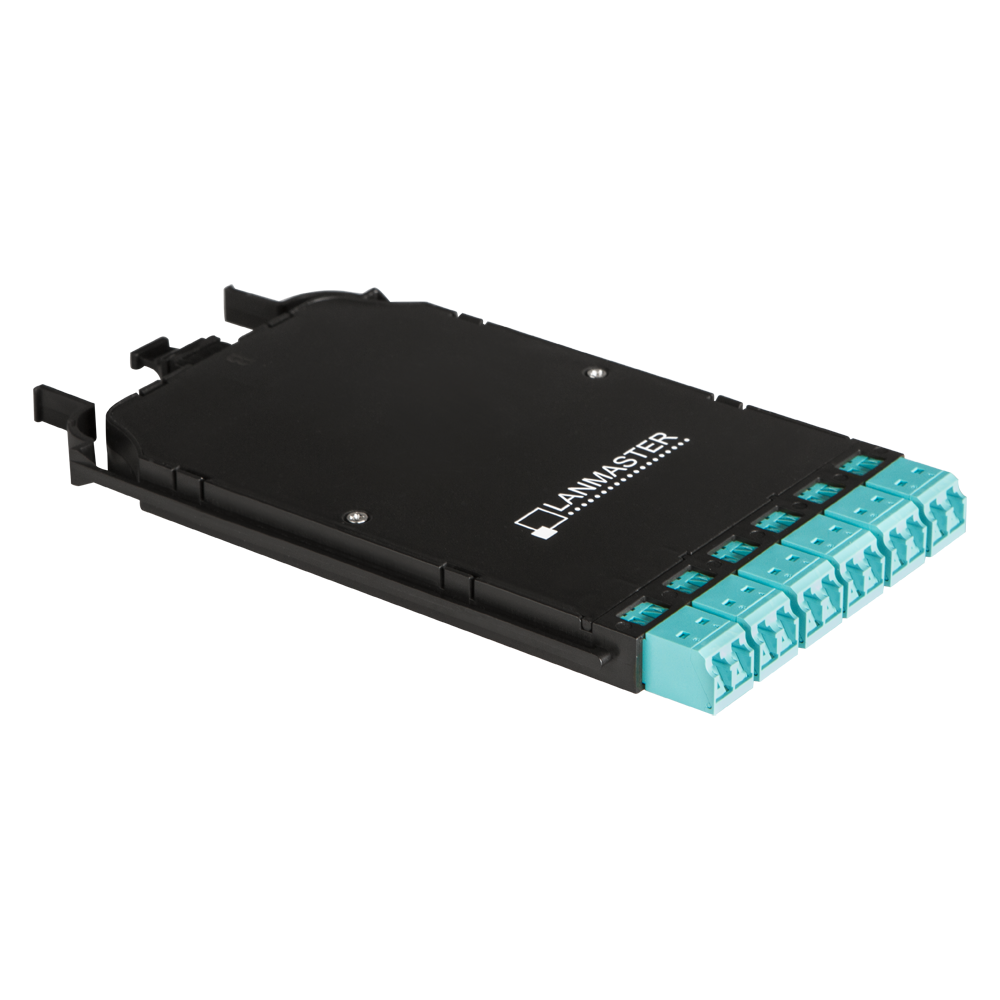
\includegraphics[width=.5\textwidth]{images/mpo-cassette.png}
   \caption{\acs{MPO} cassette}
   \label{fig:mpo-cassette}
\end{figure}
}
\slide{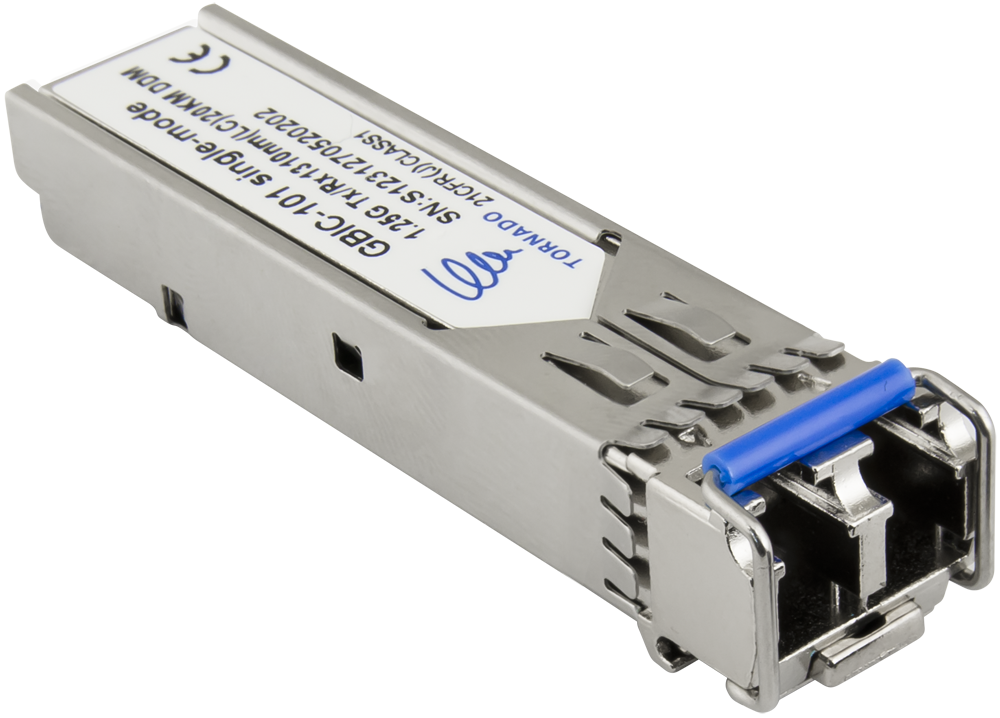
\includegraphics[width=.7\textwidth]{images/sfp.png}}
\slide{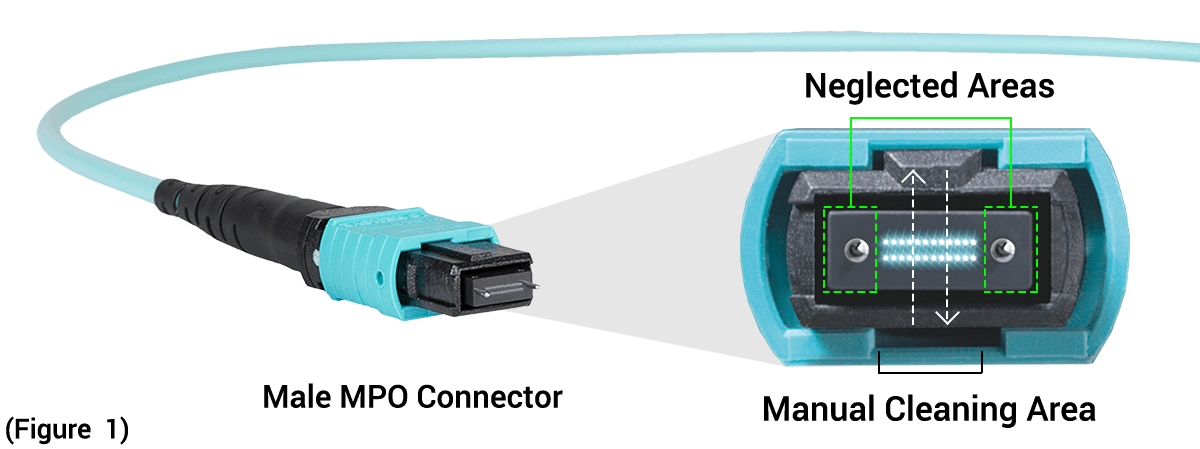
\includegraphics[width=.7\textwidth]{images/mpo.png}}
\slide{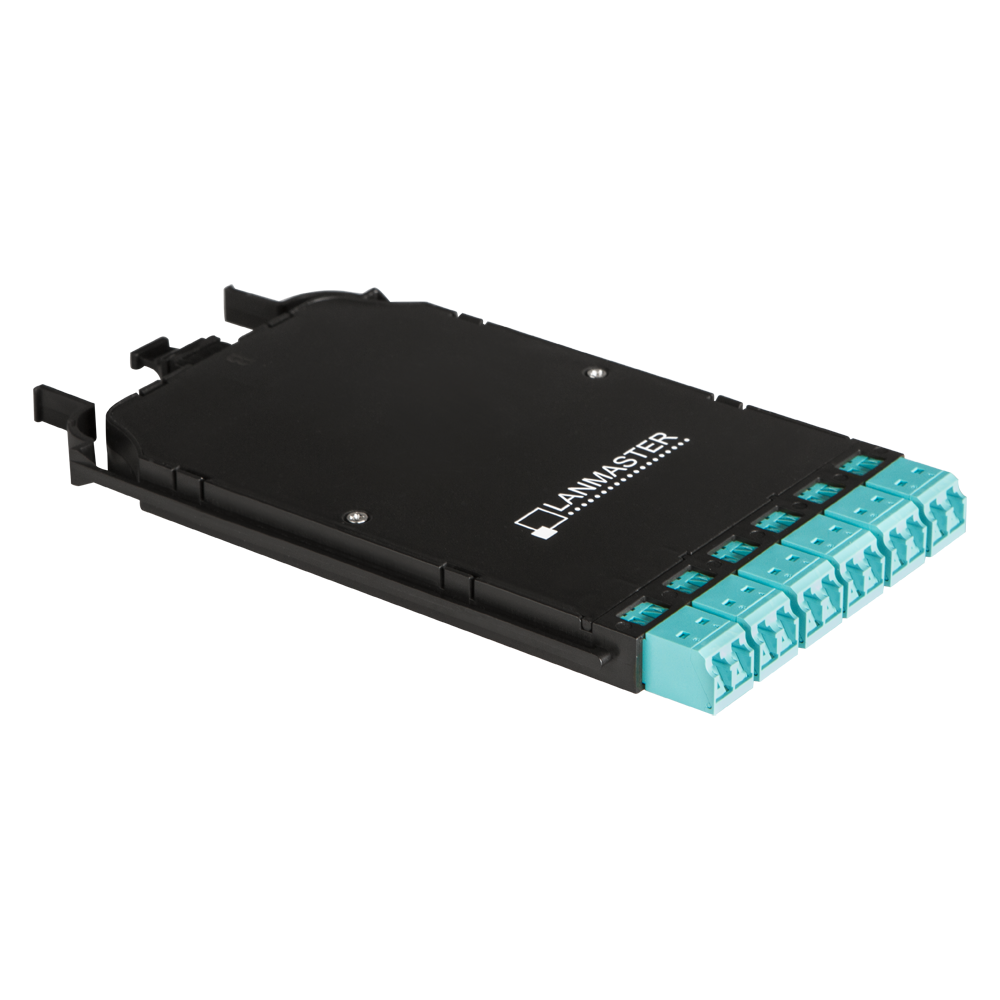
\includegraphics[width=.7\textwidth]{images/mpo-cassette.png}}






\Section{Wireless}
\label{sec:wireless}

\Paragraph{802.11}
\mode<article>{
\acs{IEEE} 802.11 specifies the set of \acf{MAC} and physical layer (\abbr{PHY}) protocols for implementing \acf{WLAN} computer communication.
The standard and amendments provide the basis for wireless network products using the Wi-Fi brand and are the world's most widely used wireless computer networking standards.

\begin{table}
   \centering
   \sffamily
   \begin{tabular}{lrrrl}
   \textbf{standard} & \textbf{generation} & \textbf{max linkrate}   & \textbf{adoption} & \textbf{frequency} \\
                     &                     & {\small \textbf{(Mbps)}} &                   & {\small \textbf{(GHz)}} \\[1ex]
   802.11   & 0  &       2 & 1997 & 2.4 \\
   802.11a  & 2  &      54 & 1999 & 5   \\
   802.11b  & 1  &      11 & 1999 & 2.4 \\
   802.11g  & 3  &      54 & 2003 & 2.4 \\
   802.11n  & 4  &     600 & 2008 & 2.4/5 \\
   802.11ac & 5  &  6\,933 & 2014 & 5 \\
   802.11ax & 6  &  9\,608 & 2019 & 2.4/5 \\
            & 6\abbr{E} &  9\,608 & 2020 & 2.4/5/6 \\
   802.11be & 7  & 40\,000 & \emph{t.b.d.} & 2.4/5/6 \\
   \end{tabular}
   \caption{Wi-Fi generations}
   \label{fig:wifi-generations}
\end{table}
}

\Paragraph{frequency}
\mode<article>{
\acs{IEEE} 802.11 uses various frequencies including \SI{2.4}{\giga\hertz}, \SI{5}{\giga\hertz}, \SI{6}{\giga\hertz}, and \SI{60}{\giga\hertz} frequency bands.
Although \acs{IEEE} 802.11 specifications list channels that might be used, the radio frequency spectrum availability allowed varies significantly by regulatory domain.
}

\Paragraph{channel}
\mode<article>{
The \SI{2.4}{\giga\hertz} frequency supports eleven channels in the United States and thirteen channels in Europe and most of the world.
The \SI{5}{\giga\hertz} frequency supports over fifty channels, depending on the bandwidth used.

\begin{figure}
\centering
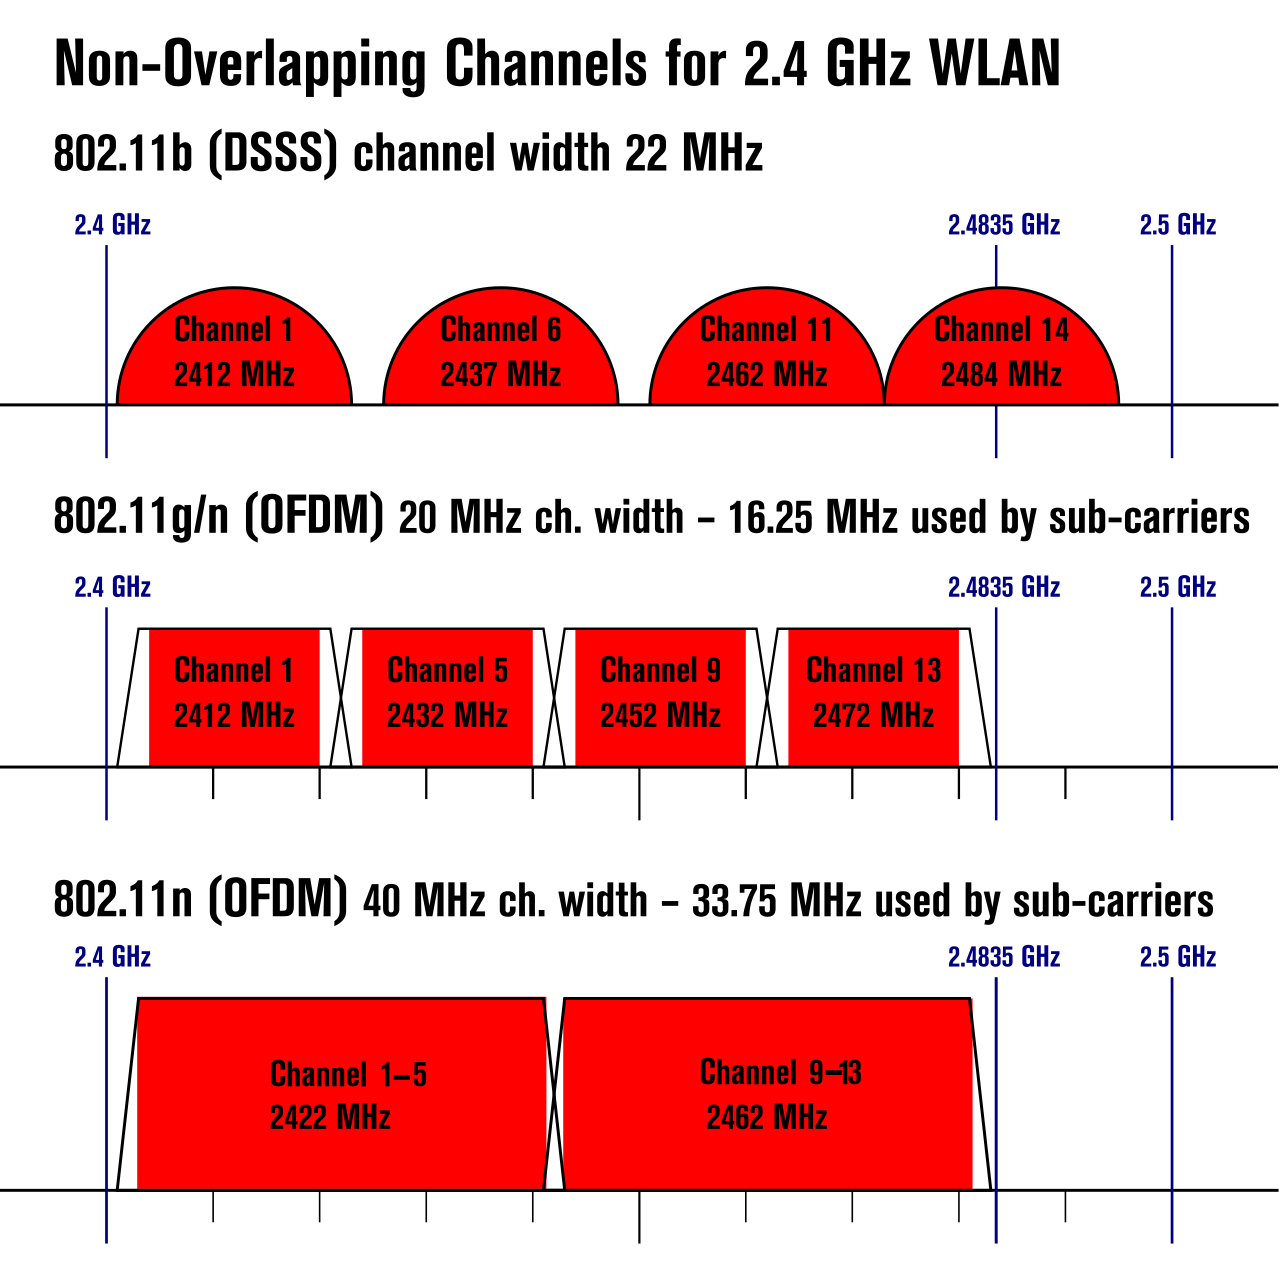
\includegraphics[width=.7\textwidth]{images/wifi-channels.png}
\caption{Non-overlapping wireless channels in the \SI{2.4}{\giga\hertz}-range}
\label{fig:wifi-channels}
\end{figure}
}

\Paragraph{bandwidth}
\mode<article>{
The bandwidth is one of the determinants of the capacity of a given communication channel.
Using a wireless channel with a bandwidth of \SI{40}{\mega\hertz} results in bigger speeds than a bandwidth of \SI{20}{\mega\hertz}.
However, when choosing the bandwidth, you have to make sure all devices that must connect to the wireless network do support this higher bandwidth.
}

\Paragraph{SSID}
\mode<article>{
The \ac{SSID} defines a service set or extended service set.%
\footnote{An \ac{ESS} is a wireless network, created by multiple access points, which appears to users as a single, seamless network, such as a network covering a home or office that is too large for reliable coverage by a single access point.}
Normally it is broadcast in the clear by stations in beacon packets to announce the presence of a network and seen by users as a wireless network name.
}

\Paragraph{antennas}
\mode<article>{
Professional access points are designed to be mounted upside down on the ceiling.
They radiate down into the room for a few metres and try to cover as much space on the floor as possible.
They are not designed to radiate upwards to the above floor or far down, to reach the floor below.

If you want to use such an access point to cover a large area in a garden, you would have to connect a different, external, antenna with a different coverage area.
}

\Paragraph{security}
\mode<article>{
Wi-Fi security includes \ac{WEP} and \ac{WPA}.
\ac{WEP} is a notoriously weak security standard: the password it uses can often be cracked in a few minutes with a basic laptop computer and widely available software tools.

There are two options available when chosing \ac{WPA}: personal mode and enterprise mode.
\ac{WPA} personal is also referred to as \acs{PSK} or \acl{PSK}.
This mode is designed for home and small office networks and does not require an authentication server.
Instead all users can access the wireless network using a common \acl{PSK}.

\ac{WPA} enterprise or \abbr{802.1X} requires a \ac{RADIUS} server for authentication.
This mode requires a more complicated setup, but provides additional security (e.g.\ protection against dictionary attacks on short passwords).
Most noticably, it requires users to authenticate to the wireless network using both a username and a password.
Often the credentials required are the same as the credentials required to access your company computer and thus Windows can authenticate to the wireless network automatically.

\ac{WPS} is an alternative authentication key distribution method intended to simplify and strengthen the process, but which, as widely implemented, creates a major security hole via \ac{WPS} \abbr{PIN} recovery.
}

\mode<article>{
\section{Further reading}
\textcite{oliviero} covers cables in quite a bit of detail and \textcite{coleman} covers wireless networks.
}